\chapter{بخش پنجم}
در این قسمت یک کنترل‌کننده PID دو درجه آزادی برای سیستم طراحی شد که خروجی خطی و غیرخطی آورده شده است.
\begin{figure}[H]
	\centering
	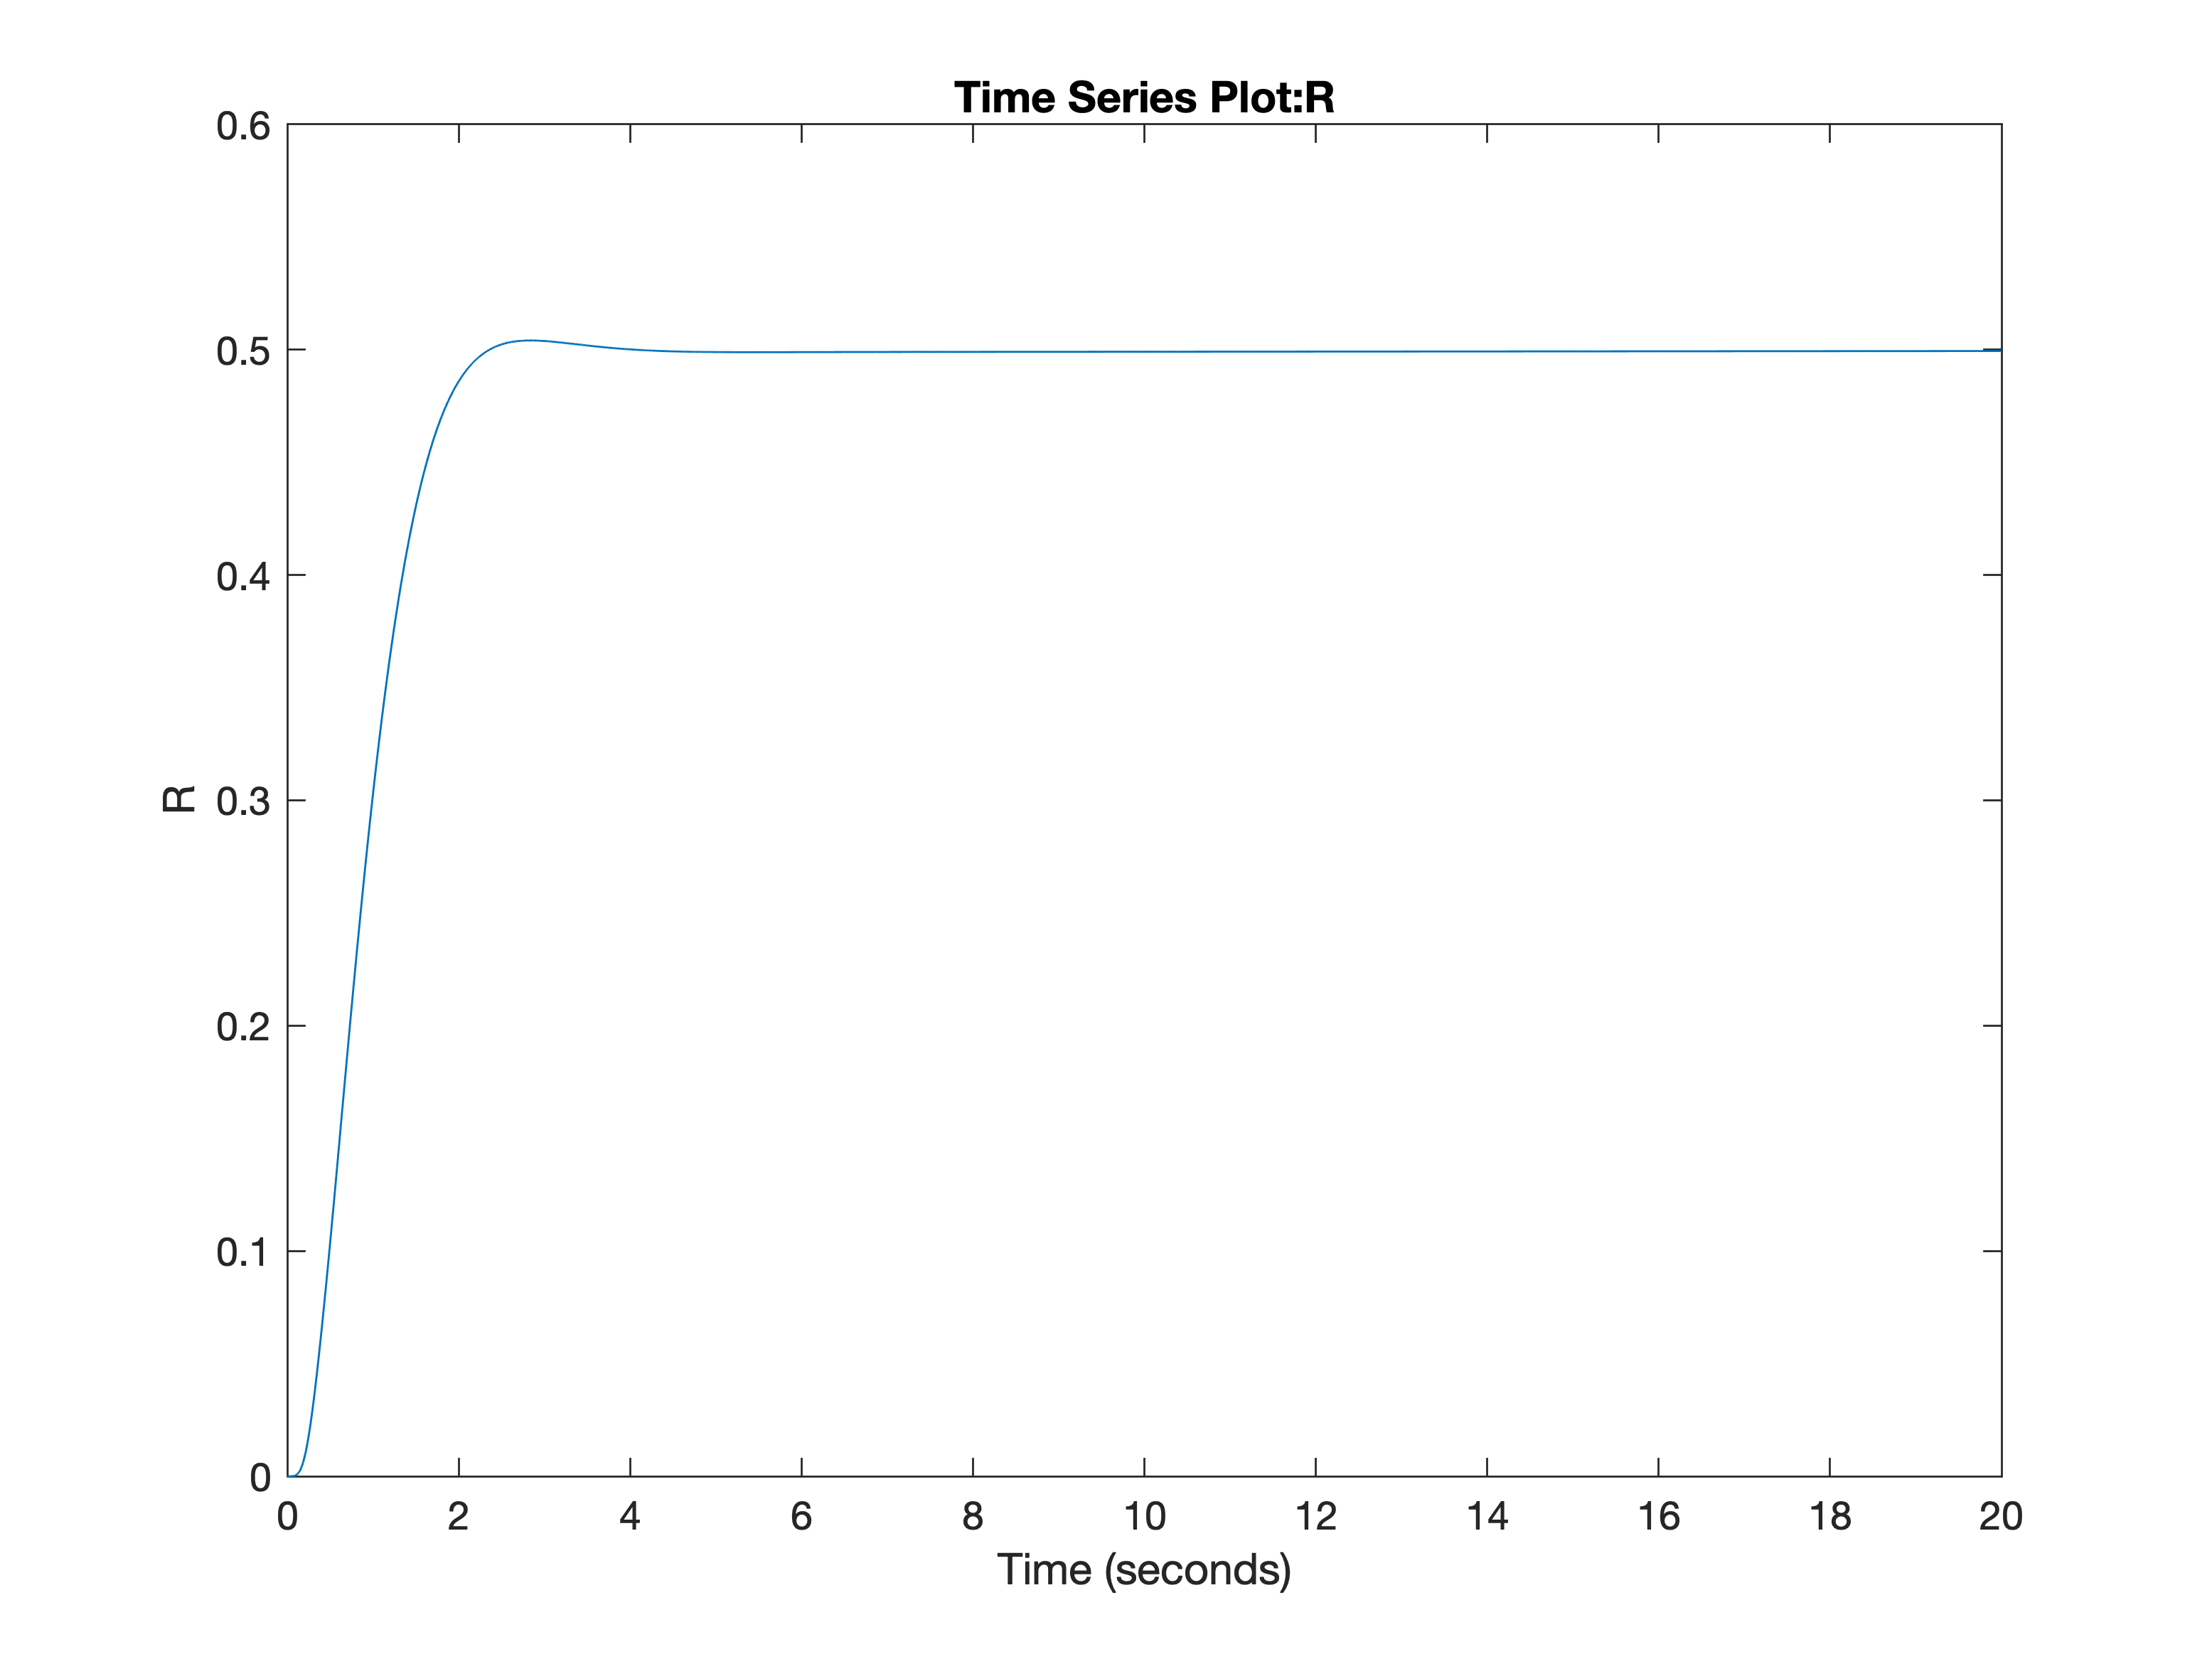
\includegraphics[width=12cm]{../Figure/P_V/PID2DOF.png}
	\caption{پاسخ پله سیستم در حضور کنترل‌کننده دو درجه آزادیPID طراحی شده }
\end{figure}
در ادامه به پیاده سازی کنترل‌کننده دو درجه ازادی طراحی شده در این بخش برروی مدل غیر خطی پرداخته می شود که در این مورد نیز گنترلر را در دو حالت با / بدون بلوک اشباع به مدل غیر خطی اعمال شده است که نمایی از بلوک دیاگرام این دو حالت در سیمولینک و انیمیشن حرکت توپ به صورت زیر است:
%
\begin{figure}[H]
	\centering
	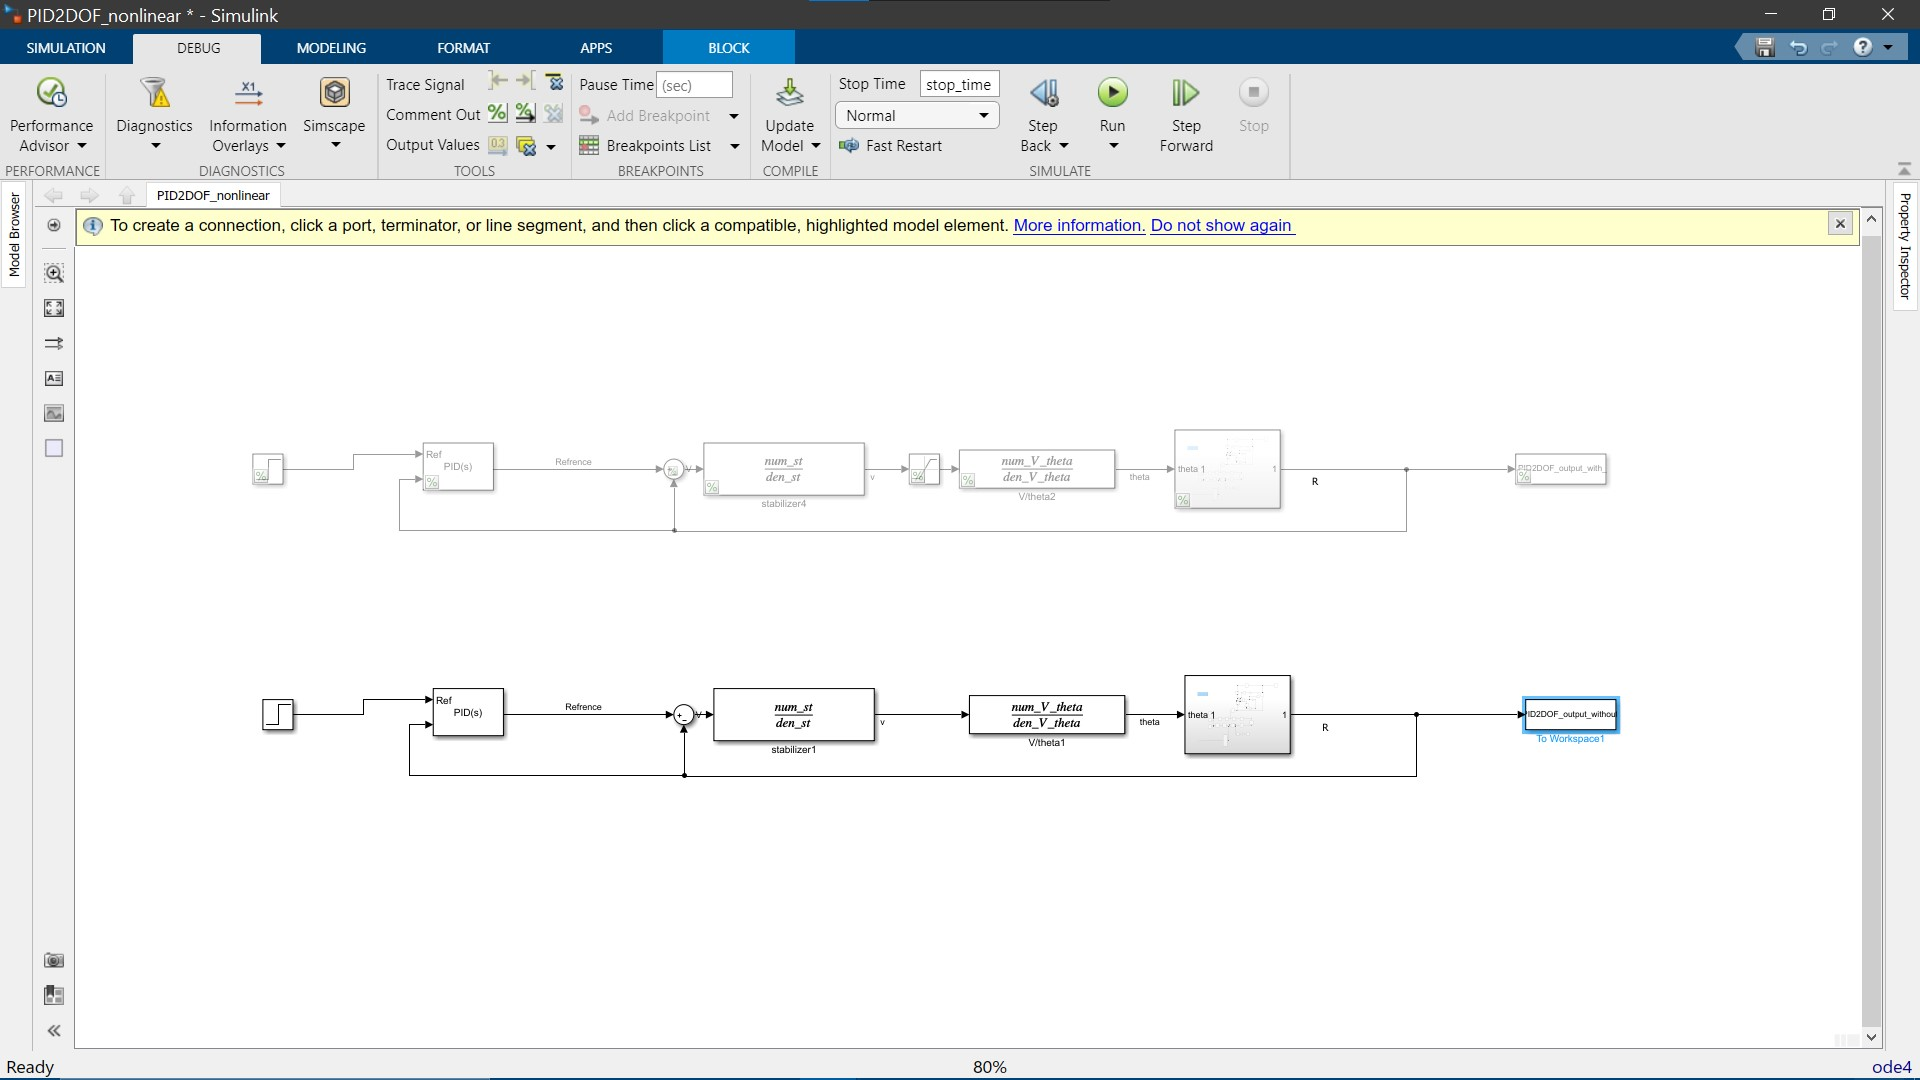
\includegraphics[width=12cm]{../Figure/P_V/PID_2DOF_NONLINEAR_SIMULINK.jpg}
	\caption{بلوک دیاگرام پیاده سازی کنترل‌کننده دو درجه آزادی بر روی مدل غیر خطی در دو حالت با / بدون بلوک اشباع}
\end{figure}

\begin{figure}[H]
	\centering
	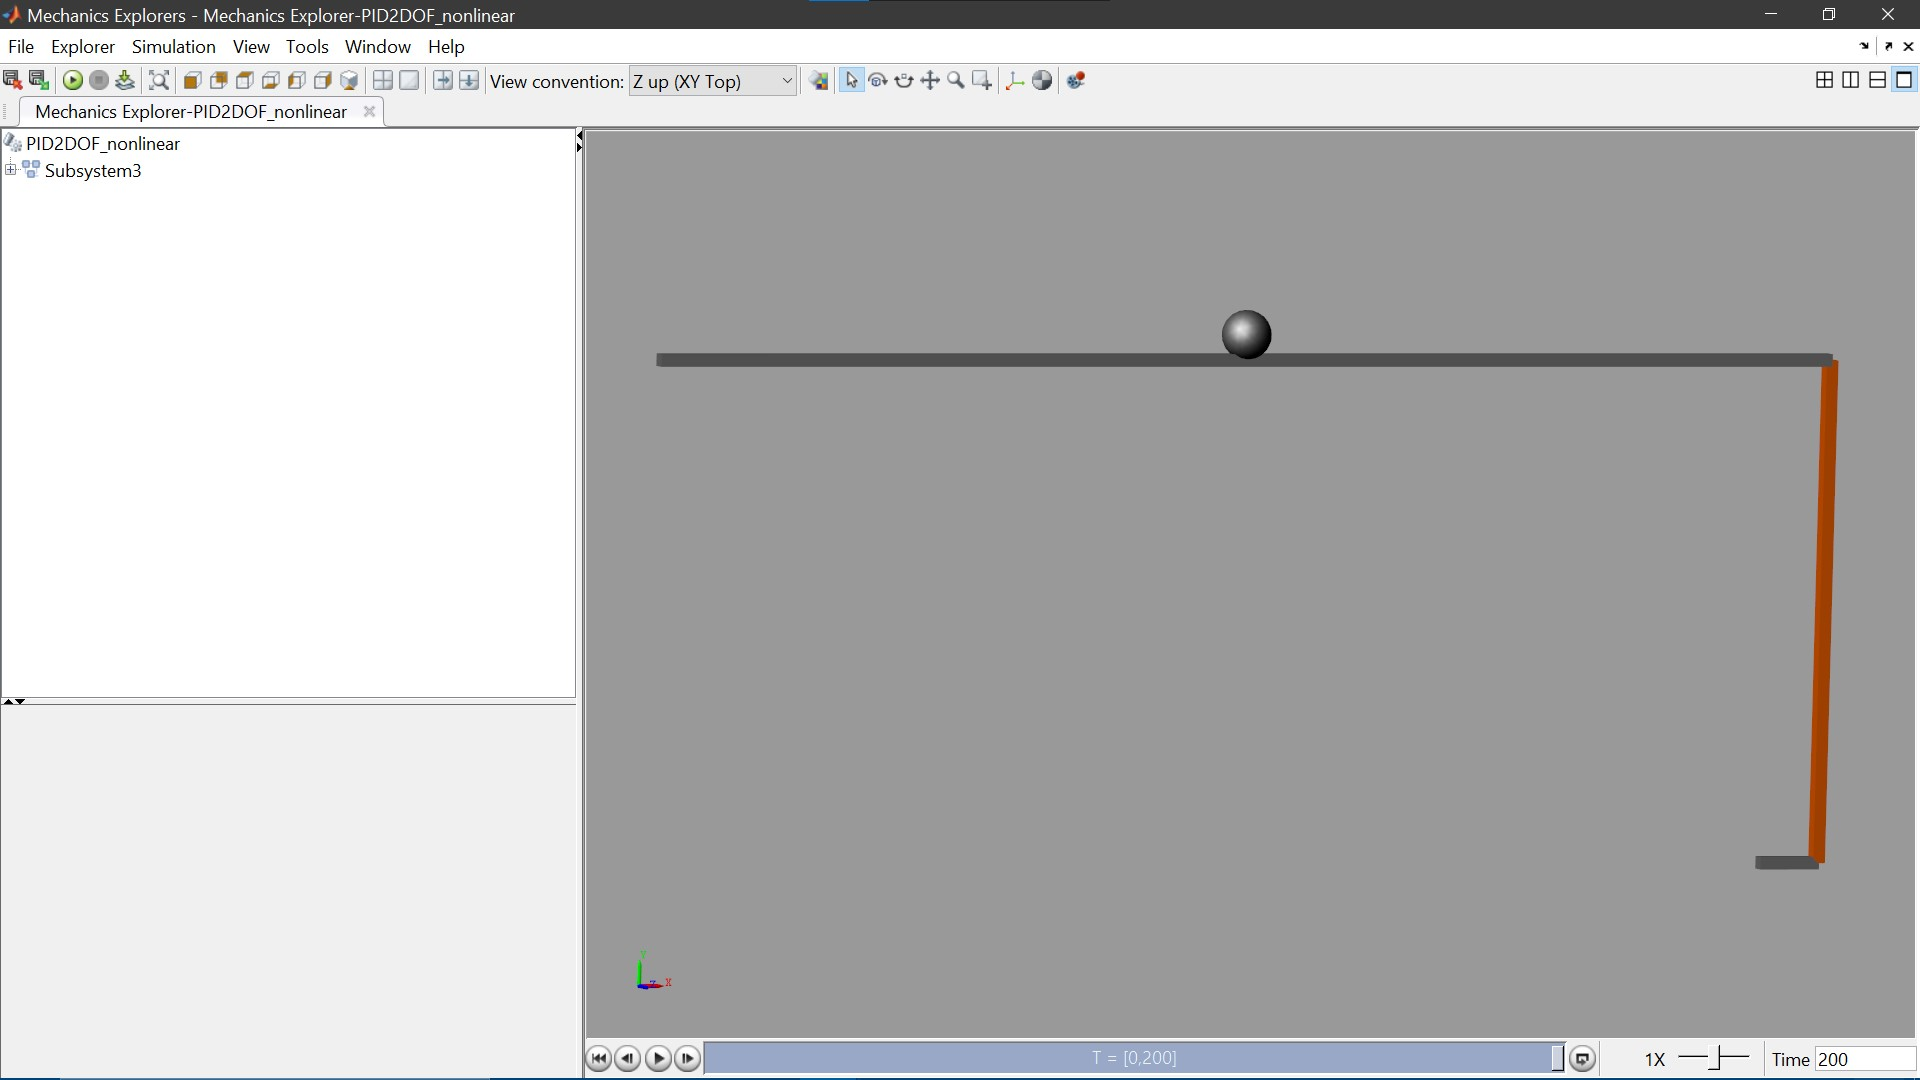
\includegraphics[width=12cm]{../Figure/P_V/PID_2DOF_nonlinear_simmechanic.jpg}
	\caption{بلوک دیاگرام پیاده سازی کنترل‌کننده دو درجه آزادی بر روی مدل غیر خطی در دو حالت با / بدون بلوک اشباع}
\end{figure}



که خروجی انها در هر یک از دو حالت بالا به صورت زیر است:
%
\begin{figure}[H]
	\centering
	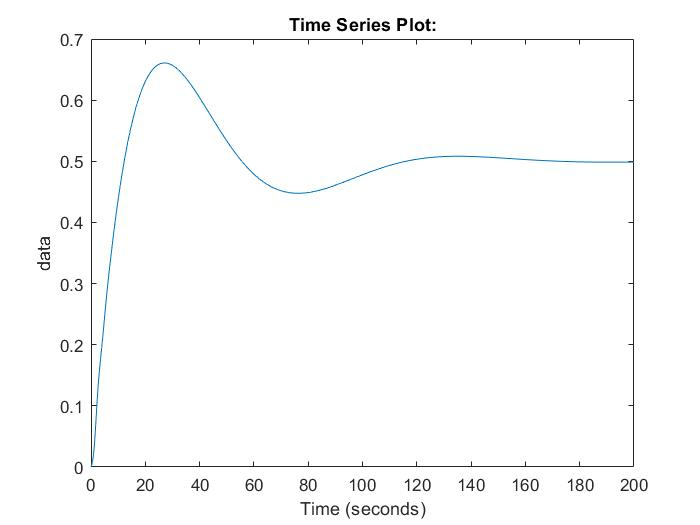
\includegraphics[width=12cm]{../Figure/P_V/PID_2DOF_OUTPUT_WITH_SATURATIO.jpg}
	\caption{خروجی سیستم با کنترل‌کننده دو درجه ازادی پیاده سازی شده بر روی سیستم غیر خطی با بلوک اشباع}
\end{figure}

\begin{figure}[H]
	\centering
	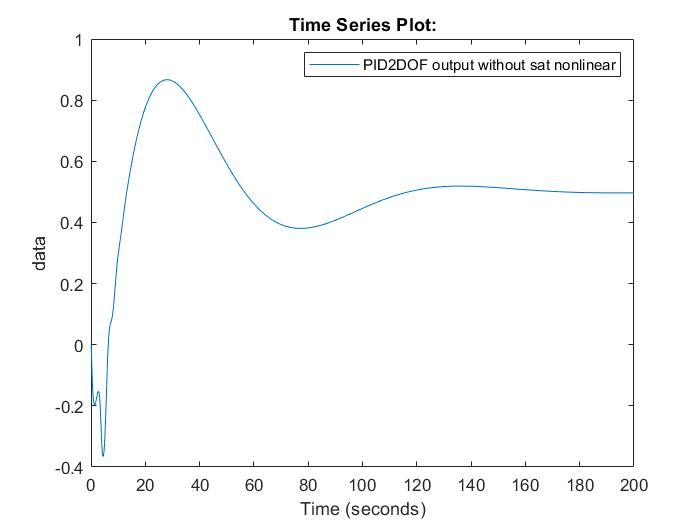
\includegraphics[width=12cm]{../Figure/P_V/PID2DOF output without sat nonlinear.jpg}
	\caption{خروجی سیستم با کنترل‌کننده دو درجه ازادی پیاده سازی شده بر روی سیستم غیر خطی بدون بلوک اشباع}
\end{figure}



همانطور که ملاحظه می شود در هر دو حالت بالا با پیاده سازی کنترل‌کننده بر روی مدل غیر خطی زمان نشست به بیشتر از 100 ثانیه افزایش یافته است